\subsection{View}

In \autocite{krasner-pope-88}, Krasner and Pope described an application's view as the graphical representation of an application's model. Several mock-ups are made to better visualize how the user interface should be structured using a UI design tool called Figma.  


\subsubsection{Rule Management Form}

To facilitate the validation rule management functionality described in \autoref{subsection:management}, a page containing a form to create, edit, delete and read a validation rule will be created. The rule management form is intended to be used by internal employee, preferably with technical background\footnote{An understanding on how HTTP works is a prerequisite to use the form} to manage a validation rule that will be used to validate a customer.

\begin{figure}[!h]
 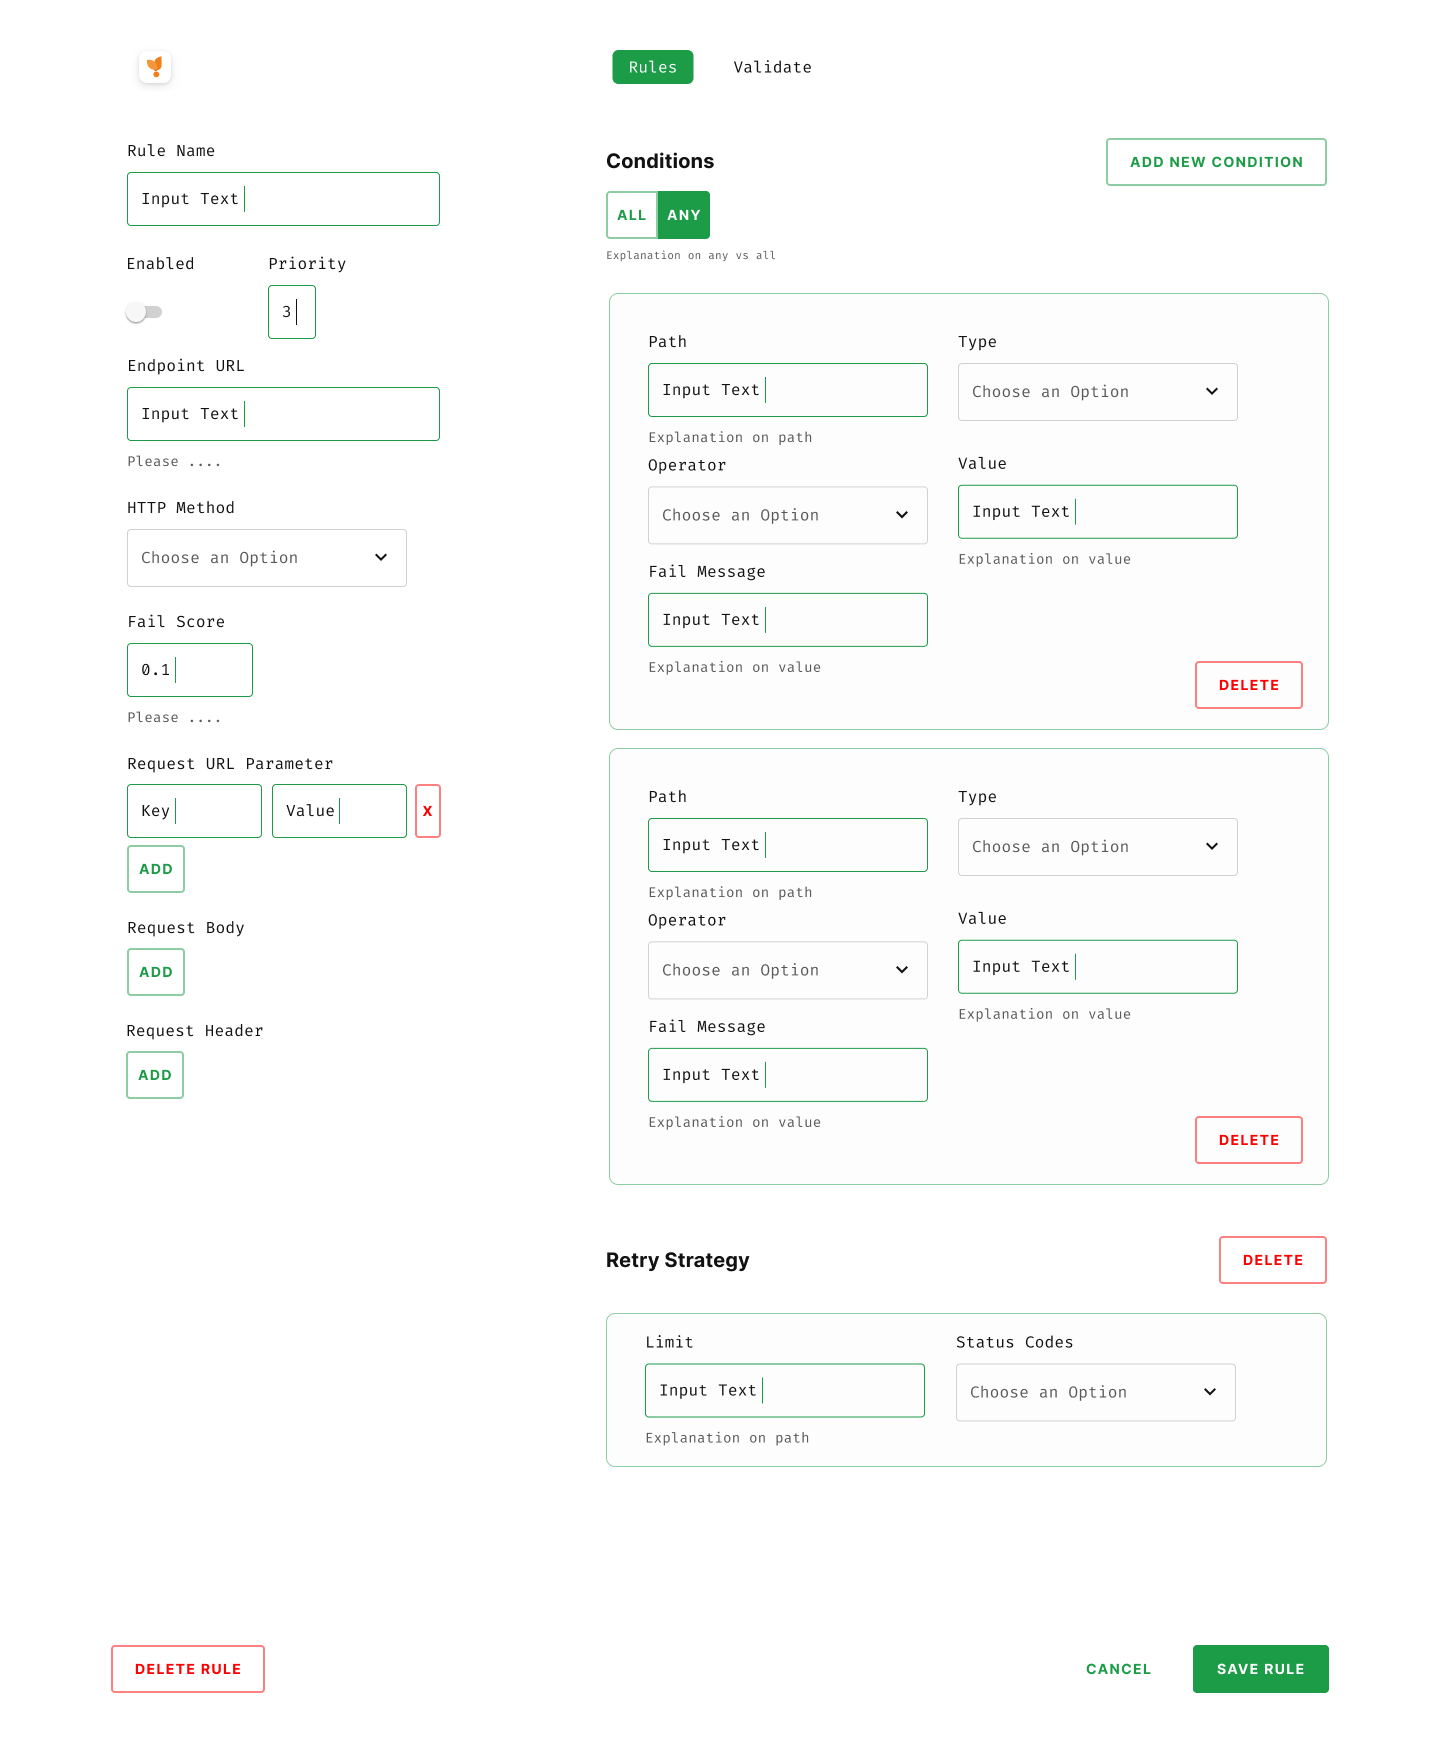
\includegraphics[width=\textwidth]{diagrams/mockup_rule_management.png}
 \caption{Mock up of the rule management form page}
\end{figure}

The page should represent every attribute of a validation rule and gives the user the ability to modify the attribute if necessary. The above listed form will be used both for rule creation and rule modification. For a rule creation, the form fields will be left blank. For a rule modification, the form fields will be filled with the rule's current data. 

The \textsc{Rule Name} field is used to display or enter a unique name of the validation rule. If the form is used to modify an existing rule, the field should be disabled, as a validation rule's name cannot be modified. 

The \textsc{Conditions} section can be used to add one or more condition to a validation rule. As described in \autoref{subsub:rule}, the form fields of each condition includes a dedicated input field for each attribute of a condition. The \textsc{Type} and \textsc{Operator} form fields are a selectable field, meaning the user has to select one out of several choices provided. This is intended to restrict input from the user, preventing an invalid condition being submitted to the FDS\footnote{For example, on \emph{type} field, user can only choose on of the following: (number, string, array, boolean)}. User can also delete a condition if necessary by clicking the \textsc{Delete} button available on each condition segment. If more than one condition is present, a selectable button will be displayed to select whether the "any" or "all" condition will be used. 

As the \emph{retryStrategy} attribute of a validation rule is not required, it is possible to delete an existing retry strategy, by clicking on the \textsc{Delete} button available on the \textsc{Retry Strategy} section of the form. If no retry strategy is present, a button to add a new retry strategy and to display the \textsc{Limit} and \textsc{Status Codes} fields will be displayed.

According to the model of a validation rule, \emph{requestBody, requestHeader} and \emph{requestUrlParameter} should be a dictionary that could contain as many entries as possible. To mimic this functionality as a form field, the \textsc{Request Body, Request Header} and \textsc{Request URL Parameter} fields are a dynamic input field. A dynamic input field enables the user to add a new key-value pair to the dictionary by clicking on the \textsc{Add} button and inputting the values to the corresponding input fields. To delete an entry of a dictionary, a delete button is provided next to each key-input fields. 


\subsubsection{Validation Form}

\begin{figure}[!h]
 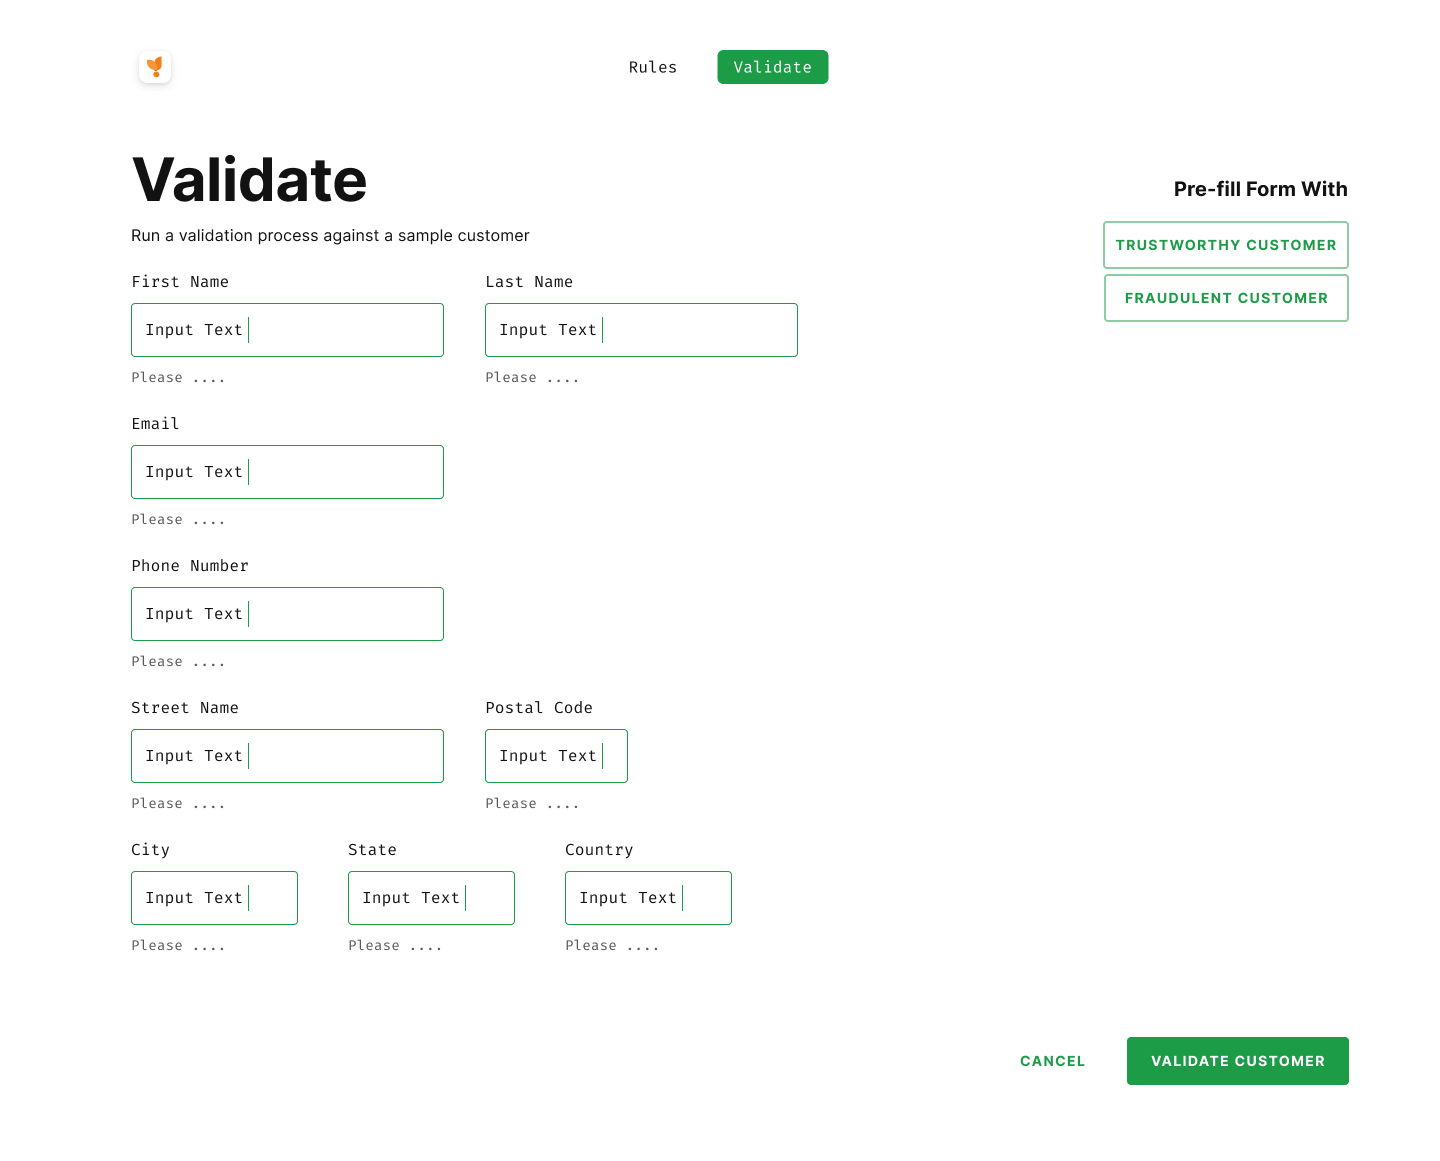
\includegraphics[width=\textwidth]{diagrams/mockup_validation_form.png}
 \caption{Mock up of the validation form page}
\end{figure}

A sample registration form is also created to give the user a possibility to run a validation process on a certain customer. The validation form is intended to be used by end customer, as a mean to register his-/herself into the system. Internal employees can also use the validation form to test the validation rules made.

The page should represent a customer model by displaying every attribute of a customer in a form field. \textbf{TODO: link to appendix -> customer UML?}. For demonstration purposes, it might be beneficial to have a list of sample customers, so that the user can run a validation on a certain set of customers quickly, without having to first fill out the form by him-/herself. To provide this functionality, a list of buttons, containing a description text of the sample customer will be displayed next to the validation form. Upon clicking on one of the button, the validation form will be filled with the sample customer's data and the user can directly click on the \textsc{Validate Customer} button to begin the validation process.


\newpage
\subsubsection{Validation Progress}

To provide a transparency on an asynchronous validation process, a page that displays the current progress of a validation process in real time might be beneficial. This page is intended for demonstration purposes, but can also be beneficial for security agents to keep track of the validation processes run by the FDS.

\begin{figure}[!h]
 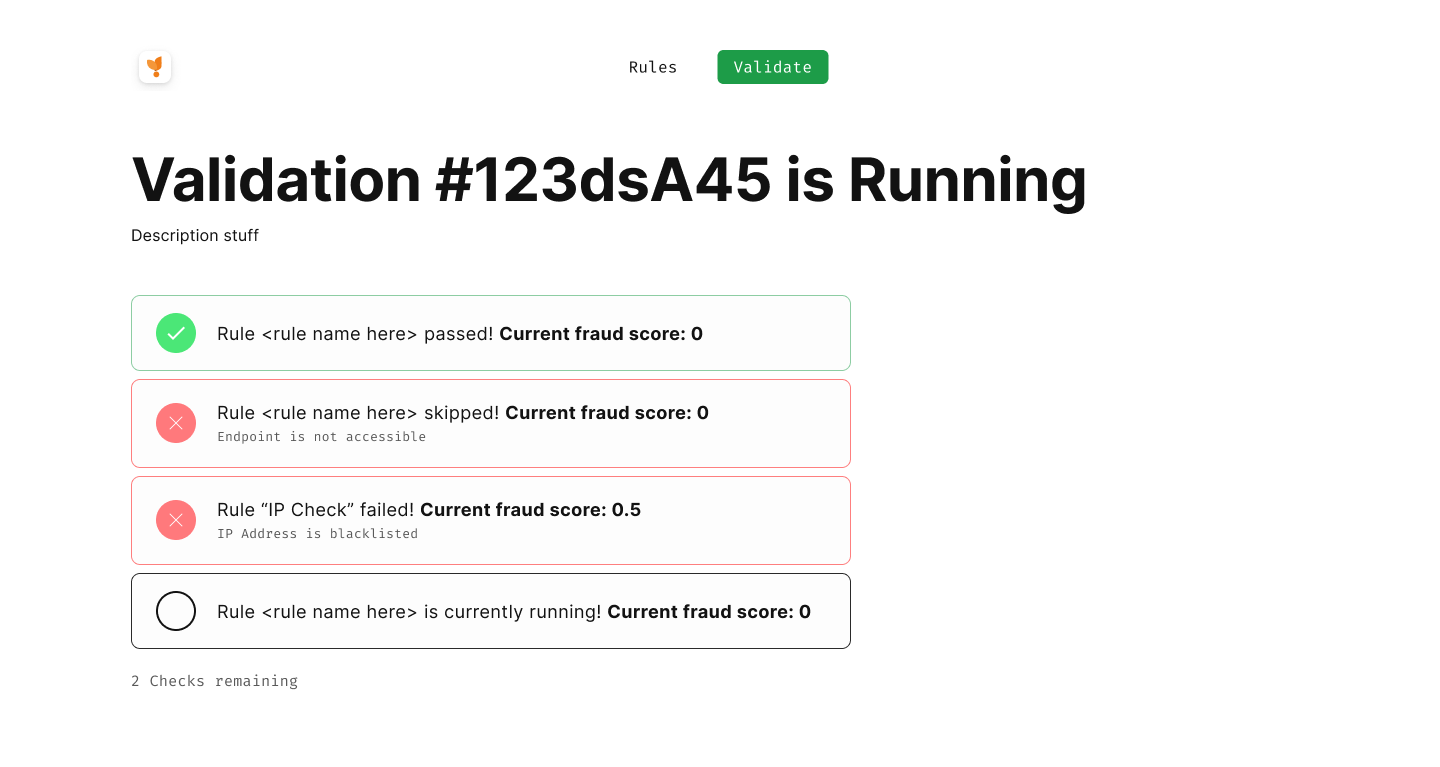
\includegraphics[width=\textwidth]{diagrams/mockup_validation_progress.png}
 \caption{Mock up of the validation progress page}
\end{figure}

The page displays the current progress of a certain validation in real time. It represents the \emph{events} attribute of a validation result in a timeline, displaying the events in a list ordered by its \emph{dateEnded} attribute. The page gives the user information regarding the evaluation result of each validation rule (either success or failure), the current fraud score and the names of validation rules that are skipped. If present, the messages of an event should also be displayed. 